\documentclass[12pt]{article}
\usepackage{graphicx}
\usepackage{dcolumn}
\usepackage{lscape}
\usepackage{amsmath}
\usepackage{listings}
\usepackage{color}

\definecolor{dkgreen}{rgb}{0,0.6,0}
\definecolor{gray}{rgb}{0.5,0.5,0.5}
\definecolor{mauve}{rgb}{0.58,0,0.82}

\lstset{frame=tb,
  language=Java,
  aboveskip=3mm,
  belowskip=3mm,
  showstringspaces=false,
  columns=flexible,
  basicstyle={\small\ttfamily},
  numbers=none,
  numberstyle=\tiny\color{gray},
  keywordstyle=\color{blue},
  commentstyle=\color{dkgreen},
  stringstyle=\color{mauve},
  breaklines=true,
  breakatwhitespace=true,
  tabsize=3
}

\begin{document}
\begin{center} 
ECON 567 Assignment 2
\end{center}
\noindent Yuanxing Long\\
ID: 87017166\\
MA in Economics\\\\
\noindent Problem 1\\
\noindent I reproduce the table 1 for variables excepting $Domestic$,$Japan$, and $European$. Here the variable $space$ in my table is actually the variable $size$ in the BLP table 1. \\  
\begin{table}[!htbp] \centering 
  \caption{} 
  \label{} 
\begin{tabular}{@{\extracolsep{5pt}} cccccccc} 
\\[-1.8ex]\hline 
\hline \\[-1.8ex] 
 & year & No.model & Price & MPG & Air & Spce & HP/Wt \\ 
\hline \\[-1.8ex] 
1 & $1,971$ & $92$ & $8.856$ & $1.720$ & $0$ & $1.442$ & $0.510$ \\ 
2 & $1,972$ & $89$ & $9.042$ & $1.633$ & $0.045$ & $1.458$ & $0.407$ \\ 
3 & $1,973$ & $86$ & $9.045$ & $1.625$ & $0.070$ & $1.466$ & $0.385$ \\ 
4 & $1,974$ & $72$ & $9.254$ & $1.633$ & $0.125$ & $1.426$ & $0.368$ \\ 
5 & $1,975$ & $93$ & $9.641$ & $1.627$ & $0.108$ & $1.416$ & $0.354$ \\ 
6 & $1,976$ & $99$ & $9.490$ & $1.856$ & $0.101$ & $1.379$ & $0.354$ \\ 
7 & $1,977$ & $95$ & $9.864$ & $1.978$ & $0.084$ & $1.358$ & $0.356$ \\ 
8 & $1,978$ & $95$ & $10.602$ & $1.993$ & $0.095$ & $1.344$ & $0.363$ \\ 
9 & $1,979$ & $102$ & $10.451$ & $2.011$ & $0.088$ & $1.307$ & $0.366$ \\ 
10 & $1,980$ & $103$ & $10.726$ & $2.167$ & $0.175$ & $1.296$ & $0.363$ \\ 
11 & $1,981$ & $116$ & $13.035$ & $2.250$ & $0.241$ & $1.301$ & $0.362$ \\ 
12 & $1,982$ & $110$ & $11.591$ & $2.377$ & $0.236$ & $1.283$ & $0.358$ \\ 
13 & $1,983$ & $115$ & $11.140$ & $2.515$ & $0.200$ & $1.273$ & $0.358$ \\ 
14 & $1,984$ & $113$ & $11.647$ & $2.415$ & $0.283$ & $1.264$ & $0.387$ \\ 
15 & $1,985$ & $136$ & $12.476$ & $2.239$ & $0.331$ & $1.246$ & $0.390$ \\ 
16 & $1,986$ & $130$ & $11.782$ & $2.355$ & $0.323$ & $1.233$ & $0.398$ \\ 
17 & $1,987$ & $143$ & $13.436$ & $2.265$ & $0.392$ & $1.231$ & $0.414$ \\ 
18 & $1,988$ & $150$ & $14.885$ & $2.188$ & $0.447$ & $1.246$ & $0.432$ \\ 
19 & $1,989$ & $147$ & $16.690$ & $2.179$ & $0.503$ & $1.247$ & $0.453$ \\ 
20 & $1,990$ & $131$ & $14.038$ & $2.182$ & $0.458$ & $1.255$ & $0.449$ \\ 
\hline \\[-1.8ex] 
\end{tabular} 
\end{table} 

\newpage
\noindent I don't know how to calculate the percentiles of variable so I calculate the mean, standard error, minimum and maximum of the variables of interest. 
\begin{table}[!htbp] \centering 
  \caption{} 
  \label{} 
\begin{tabular}{@{\extracolsep{5pt}}lccccc} 
\\[-1.8ex]\hline 
\hline \\[-1.8ex] 
Statistic & \multicolumn{1}{c}{N} & \multicolumn{1}{c}{Mean} & \multicolumn{1}{c}{St. Dev.} & \multicolumn{1}{c}{Min} & \multicolumn{1}{c}{Max} \\ 
\hline \\[-1.8ex] 
model.id & 2,217 & 276.210 & 160.183 & 1 & 557 \\ 
firm.id & 2,217 & 13.744 & 6.259 & 1 & 26 \\ 
cdid & 2,217 & 11.540 & 5.741 & 1 & 20 \\ 
id & 2,217 & 2,559.081 & 1,517.647 & 129 & 5,592 \\ 
price & 2,217 & 11.761 & 8.644 & 3.393 & 68.596 \\ 
mpd & 2,217 & 2.085 & 0.698 & 0.846 & 6.437 \\ 
air & 2,217 & 0.242 & 0.428 & 0 & 1 \\ 
mpg & 2,217 & 2.100 & 0.581 & 0.913 & 5.300 \\ 
space & 2,217 & 1.310 & 0.238 & 0.756 & 1.888 \\ 
hpwt & 2,217 & 0.394 & 0.097 & 0.170 & 0.948 \\ 
trend & 2,217 & 1,981.540 & 5.741 & 1,971 & 1,990 \\ 
share & 2,217 & 0.001 & 0.001 & 0.00000 & 0.009 \\ 
outshr & 2,217 & 0.893 & 0.014 & 0.871 & 0.919 \\ 
y & 2,217 & $-$0.000 & 1.382 & $-$6.498 & 3.029 \\ 
\hline \\[-1.8ex] 
\end{tabular} 
\end{table} 
\\\\

\noindent Problem 2\\
\noindent The regression results are summarized in table 3. The regression results acquired by my codes are similar to what are reported in table 3 of BLP 1995. Calculating the elasticities of demand implied by the OLS logit model, I find that 1502 own price elasticities have absolute value less than 1.  Calculating the elasticities of demand implied by the IV logit model, I find that 430 own price elasticities have absolute value less than 1. It's more plausible to use the price elasticities implied by IV logit. The inelastic demand estimates are undesirable because the automobile in the 1980s is a luxury good, whose demand should be elastic. 

\begin{table}[!htbp] \centering 
  \caption{} 
  \label{} 
\begin{tabular}{@{\extracolsep{5pt}}lccc} 
\\[-1.8ex]\hline 
\hline \\[-1.8ex] 
 & \multicolumn{3}{c}{\textit{Dependent variable:}} \\ 
\cline{2-4} 
\\[-1.8ex] & \multicolumn{2}{c}{y} & log(price) \\ 
\\[-1.8ex] & \textit{OLS} & \textit{instrumental} & \textit{OLS} \\ 
 & \textit{} & \textit{variable} & \textit{} \\ 
\\[-1.8ex] & (1) & (2) & (3)\\ 
\hline \\[-1.8ex] 
 price & $-$0.089$^{***}$ & $-$0.158$^{***}$ &  \\ 
  & (0.004) & (0.009) &  \\ 
  & & & \\ 
 hpwt & $-$0.124 & 1.866$^{***}$ & 1.443$^{***}$ \\ 
  & (0.277) & (0.363) & (0.077) \\ 
  & & & \\ 
 air & $-$0.034 & 0.733$^{***}$ & 0.673$^{***}$ \\ 
  & (0.073) & (0.112) & (0.018) \\ 
  & & & \\ 
 mpd & 0.265$^{***}$ & 0.127$^{***}$ &  \\ 
  & (0.043) & (0.048) &  \\ 
  & & & \\ 
 mpg &  &  & $-$0.193$^{***}$ \\ 
  &  &  & (0.020) \\ 
  & & & \\ 
 trend &  &  & 0.012$^{***}$ \\ 
  &  &  & (0.001) \\ 
  & & & \\ 
 space & 2.342$^{***}$ & 2.268$^{***}$ & 0.127$^{***}$ \\ 
  & (0.125) & (0.134) & (0.042) \\ 
  & & & \\ 
 Constant & $-$2.521$^{***}$ & $-$2.291$^{***}$ & 1.667$^{***}$ \\ 
  & (0.253) & (0.270) & (0.101) \\ 
  & & & \\ 
\hline \\[-1.8ex] 
Observations & 2,217 & 2,217 & 2,217 \\ 
R$^{2}$ & 0.387 & 0.305 & 0.669 \\ 
Adjusted R$^{2}$ & 0.386 & 0.303 & 0.669 \\ 
Residual Std. Error (df = 2211) & 1.083 & 1.153 & 0.307 \\ 
F Statistic (df = 5; 2211) & 279.243$^{***}$ &  & 895.193$^{***}$ \\ 
\hline 
\hline \\[-1.8ex] 
\textit{Note:}  & \multicolumn{3}{r}{$^{*}$p$<$0.1; $^{**}$p$<$0.05; $^{***}$p$<$0.01} \\ 
\end{tabular} 
\end{table} 


\newpage
\noindent Problem 3\\
\noindent The testing result for delta.fn is summarized in the following table. Since the distribution is very close to zero, the delta function is valid.  \\
\begin{tabular}{l c  }\hline\hline
Summary of abs(delta-d.check) \\ \hline
Minimum & 2.804e-06 \\
1st Quantile  &  3.971e-06 \\
Median  & 4.338e-06 \\
Mean & 4.377e-06  \\
3rd Quantile  & 5.012e-06 \\
Maximum  & 5.235e-06 \\
\hline
\end{tabular}
\\\\\\
\noindent Next, I check whether the derivative function is right. The results as followed is distribution of difference between numerical derivative and analytical derivative. Since the distribution is very close to zero, the function should be correct. 
\begin{figure}[h!]
  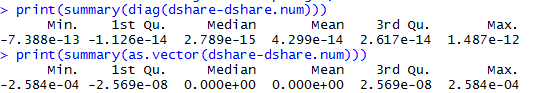
\includegraphics[width=\linewidth]{table1.png}
\end{figure}     


\newpage
\noindent Problem 4\\
\noindent The testing results are summarized in the following table. The moment function, delta.fn function and Share.fn function take most of the time.    
\begin{verbatim}
summaryRprof("blp.prof", lines="both") # show the results
$by.self
                self.time self.pct total.time total.pct
#15                  0.32    23.53       0.70     51.47
"exp"                0.26    19.12       0.26     19.12
"%*%"                0.24    17.65       0.24     17.65
#16                  0.16    11.76       0.28     20.59
"/"                  0.08     5.88       0.08      5.88
"*"                  0.06     4.41       0.06      4.41
"+"                  0.06     4.41       0.06      4.41
"as.vector"          0.04     2.94       0.18     13.24
"solve.default"      0.04     2.94       0.04      2.94
#13                  0.02     1.47       0.24     17.65
"sum"                0.02     1.47       0.02      1.47
"t"                  0.02     1.47       0.02      1.47
#14                  0.02     1.47       0.02      1.47
#25                  0.02     1.47       0.02      1.47

$by.total
                total.time total.pct self.time self.pct
"moments"             1.34     98.53      0.00     0.00
"delta.fn"            1.04     76.47      0.00     0.00
#11                   1.04     76.47      0.00     0.00
"share.fn"            1.00     73.53      0.00     0.00
#24                   1.00     73.53      0.00     0.00
#15                   0.70     51.47      0.32    23.53
#16                   0.28     20.59      0.16    11.76
"exp"                 0.26     19.12      0.26    19.12
"dshare.dp"           0.26     19.12      0.00     0.00
#17                   0.26     19.12      0.00     0.00
"%*%"                 0.24     17.65      0.24    17.65
#13                   0.24     17.65      0.02     1.47
"as.vector"           0.18     13.24      0.04     2.94
"/"                   0.08      5.88      0.08     5.88
"*"                   0.06      4.41      0.06     4.41
"+"                   0.06      4.41      0.06     4.41
"solve"               0.06      4.41      0.00     0.00
"solve.default"       0.04      2.94      0.04     2.94
#21                   0.04      2.94      0.00     0.00
"sum"                 0.02      1.47      0.02     1.47
"t"                   0.02      1.47      0.02     1.47
#14                   0.02      1.47      0.02     1.47
#25                   0.02      1.47      0.02     1.47
"matrix"              0.02      1.47      0.00     0.00
#10                   0.02      1.47      0.00     0.00
#18                   0.02      1.47      0.00     0.00

$sample.interval
[1] 0.02

$sampling.time
[1] 1.36
\end{verbatim}
Share.fn function records all the y values and then takes average. To improve efficiency, I first take the sum and then divide it by S. Similar improvement are also applied into dshare.dp function. The time is much shorter. 
\begin{verbatim}
summaryRprof("blp.prof", lines="both") # show the results
$by.self
             self.time self.pct total.time total.pct
#15               0.28    18.67       0.88     58.67
"%*%"             0.28    18.67       0.28     18.67
"exp"             0.22    14.67       0.22     14.67
"+"               0.18    12.00       0.18     12.00
"matrix"          0.16    10.67       0.16     10.67
"*"               0.08     5.33       0.08      5.33
"/"               0.08     5.33       0.08      5.33
"sum"             0.08     5.33       0.08      5.33
#16               0.04     2.67       0.24     16.00
#13               0.02     1.33       0.18     12.00
"as.vector"       0.02     1.33       0.10      6.67
"doTryCatch"      0.02     1.33       0.02      1.33
"t"               0.02     1.33       0.02      1.33
#10               0.02     1.33       0.02      1.33

$by.total
                      total.time total.pct self.time self.pct
"delta.fn"                  1.28     85.33      0.00     0.00
#3                          1.28     85.33      0.00     0.00
"share.fn"                  1.12     74.67      0.00     0.00
#24                         1.12     74.67      0.00     0.00
#15                         0.88     58.67      0.28    18.67
"%*%"                       0.28     18.67      0.28    18.67
#16                         0.24     16.00      0.04     2.67
"exp"                       0.22     14.67      0.22    14.67
"dshare.dp"                 0.20     13.33      0.00     0.00
#9                          0.20     13.33      0.00     0.00
"+"                         0.18     12.00      0.18    12.00
#13                         0.18     12.00      0.02     1.33
"matrix"                    0.16     10.67      0.16    10.67
#12                         0.16     10.67      0.00     0.00
"as.vector"                 0.10      6.67      0.02     1.33
"*"                         0.08      5.33      0.08     5.33
"/"                         0.08      5.33      0.08     5.33
"sum"                       0.08      5.33      0.08     5.33
"doTryCatch"                0.02      1.33      0.02     1.33
"t"                         0.02      1.33      0.02     1.33
#10                         0.02      1.33      0.02     1.33
".rs.callAs"                0.02      1.33      0.00     0.00
"Rprof"                     0.02      1.33      0.00     0.00
"tryCatch"                  0.02      1.33      0.00     0.00
"tryCatchList"              0.02      1.33      0.00     0.00
"tryCatchOne"               0.02      1.33      0.00     0.00
"withCallingHandlers"       0.02      1.33      0.00     0.00

$sample.interval
[1] 0.02

$sampling.time
[1] 1.5
\end{verbatim}        

\newpage
\noindent Problem 5\\
\noindent The estimates are not very similar to the Table 4 of BLP 1995. Most of betas have the same sign as in the paper but most of gammas don't have the same sign as in the paper. It implies that I correctly estimated the demand side parameters but not the cost side parameters. 

\begin{table}[!htbp] \centering 
  \caption{} 
  \label{} 
\begin{tabular}{@{\extracolsep{5pt}} cc} 
\\[-1.8ex]\hline 
\hline \\[-1.8ex] 
alpha & $20.440$ \\ 
sigma.constant & $0.361$ \\ 
sigma.hpwt & $4.816$ \\ 
sigma.air & $0.200$ \\ 
sigma.mpd & $0.659$ \\ 
sigma.space & $0.330$ \\ 
beta.constant & $$-$11.216$ \\ 
beta.hpwt & $$-$1.088$ \\ 
beta.air & $4.891$ \\ 
beta.mpd & $0.293$ \\ 
beta.space & $5.536$ \\ 
gamma.constant & $1.951$ \\ 
gamma.hpwt & $$-$0.064$ \\ 
gamma.air & $1.353$ \\ 
gamma.mpd & $0.535$ \\ 
gamma.space & $0.376$ \\ 
gamma.trend & $$-$0.021$ \\ 
\hline \\[-1.8ex] 
\end{tabular} 
\end{table} 

\newpage
\noindent The estimated own and cross-price semi-elasticities are summarized in the following table. It's slightly different from the elasticities in the paper.  
\begin{figure}[h!]
  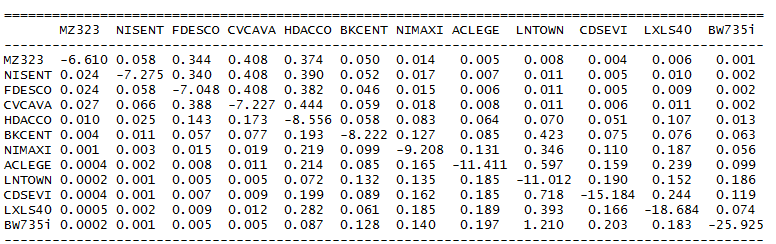
\includegraphics[width=\linewidth]{table2.png}
\end{figure}     

\newpage
\noindent Problem 6\\
\noindent The standard errors for our estimates are summarized in the following table.  
\begin{table}[!htbp] \centering 
  \caption{} 
  \label{} 
\begin{tabular}{@{\extracolsep{5pt}} ccc} 
\\[-1.8ex]\hline 
\hline \\[-1.8ex] 
 & estimate & sd \\ 
\hline \\[-1.8ex] 
alpha & $20.440$ & $0.057$ \\ 
sigma.constant & $0.361$ & $0.0004$ \\ 
sigma.hpwt & $4.816$ & $0.0001$ \\ 
sigma.air & $0.200$ & $0.00001$ \\ 
sigma.mpd & $0.659$ & $0.0001$ \\ 
sigma.space & $0.330$ & $0.001$ \\ 
beta.constant & $$-$11.216$ & $0.962$ \\ 
beta.hpwt & $$-$1.088$ & $3.348$ \\ 
beta.air & $4.891$ & $0.460$ \\ 
beta.mpd & $0.293$ & $0.184$ \\ 
beta.space & $5.536$ & $0.505$ \\ 
gamma.constant & $1.951$ & $0.154$ \\ 
gamma.hpwt & $$-$0.064$ & $0.116$ \\ 
gamma.air & $1.353$ & $0.136$ \\ 
gamma.mpd & $0.535$ & $0.169$ \\ 
gamma.space & $0.376$ & $0.179$ \\ 
gamma.trend & $$-$0.021$ & $0.005$ \\ 
\hline \\[-1.8ex] 
\end{tabular} 
\end{table} 

 

\end{document}